\section{Artificial Neural Networks}

Artificial nerual networks are a type of artificial intelligence that can be used to classify data and be implemented in software. There are inumerable architectures for a neural network however they all feature some common characteristics and each is designed to perform a single specific task. Generally speaking a neural network receives in input to which it responds by producing an output, for example a neural network could receive an image of a bowl of fruit and be designed to tell you if there are any bananas present. Figure \ref{fig:neural_network} outlines the basic structure of a neural network, which is comprised of three layers. The input layer interacts directly with the input, the output layers produces the final output and the middle layer of neurons is described a 'black box' because its behaviour is not fully understood. The input and output patterns refer to a regularity in data that the neural network attempts to recognise and use to take action like classifying data into groups\cite{statistical_pattern_recognition}. 


\begin{figure}[h]
    \centering
    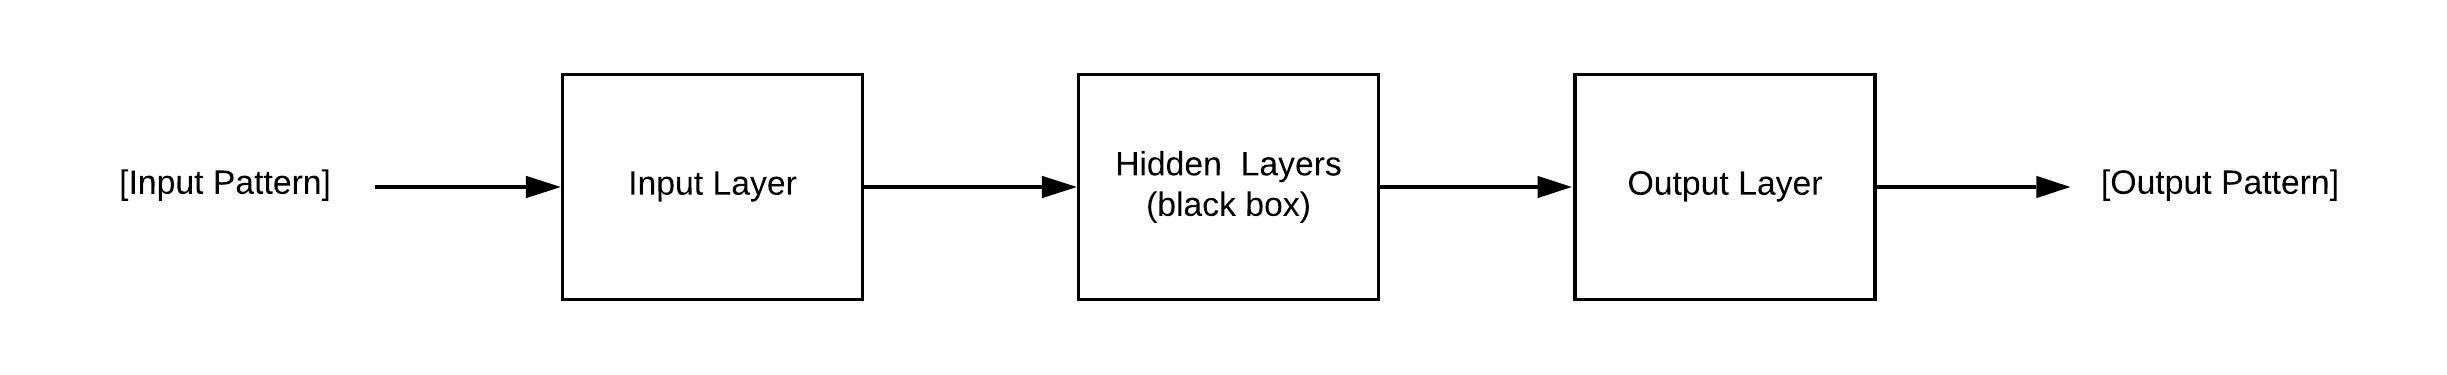
\includegraphics[width = 0.9\textwidth]{litreview/computervision/neuralnetworks/neural_network_basic_structure}
    \caption{Basic structure of a neural network \cite{neural_networks}.}
    \label{fig:neural_network}
\end{figure}

\subsubsection{Neurons}

The layers Neural networks are comprised of a fundamental unit called a neuron. Each neuron is comprised of an activiation function, a bias and a weight. An activiation function determines the output of a neuron as a function of its inputs, the simplest activation function is a step function, meaning that if the sum of the inputs is less than some threshold then the output of the neuron is 0, otherwise it's 1 \cite{machine_learning_dictionary}. A neuron's weight scales its output value when it's passed as an input to another neuron and thus alters the influence of a neuron's output on the entire neural network's output. A neuron's bias is a value that is added to the neuron's output. The bias is a trainable quantitiy meaning that it can be changed in order to change the behaviour of a neural network, however not all neural networks use biases \cite{neural_networks}. Figure \ref{fig:neuron} provides a diagram of a neuron outlining all of its components, inputs and outputs. 


\begin{figure}[h]
    \centering
    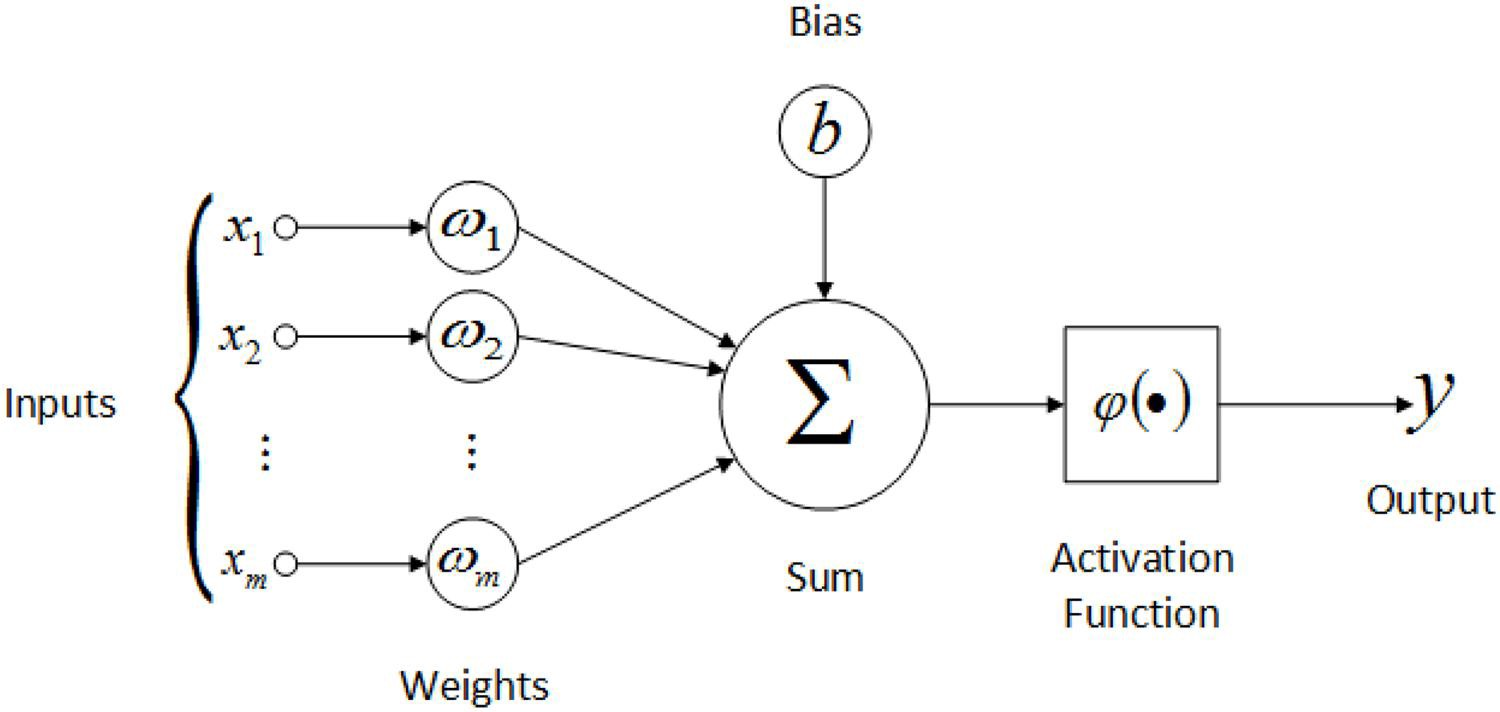
\includegraphics[width = 0.8\textwidth]{litreview/computervision/neuralnetworks/neuron}
    \caption{An artificial neuron \cite{ann_handbook}.}
    \label{fig:neuron}
\end{figure}

A single neuron on its own does not accomplish a lot however, given a large number of interacting neurons with weighting's and activiation function configured to recognise a specific pattern the desired output for a given input can be achieved.

\subsubsection{Data Aqcuisition and Training}

The process of determining the weightings of a neural network which in term determine its behaviour is achieved via \emph{training}. In training a neural network it is passed data samples and its response to them is observed, according to this response its weightings to improve the accuracy of its responses. All methods of network training require sample data test the network, for comprehensive computer vision applications in particular the amount of data required is very large \cite{large_data_neural_network}. In addition to collecting data ofttimes the samples require labelling so that the network may be given more specific adjustments whilst it's trained. A sufficiently large amount of time must be spent collating and preparing data just to train a neural network \cite{data_labelling} that it can be regarded as disadvantage.

The execution of a training algorithm can also take a large amount of time dpeendent on the complexity of the network's activation functions and the amount of data required, these factors can make the requisite computation power to utilize a neural network, even after its trained, prohibitive for low power machines like microcontrollers \cite{computations_neural_network}. 

A simple method of evaluating a network's success at classifying data is to observe the ratio of successful classifications to unsuccessful ones. Evaluation becomes more complex when you consider not the absolute number of of classifications but the classification of individual data samples and whether or not they were correct. For a binary classification (just two classes) these measurements are referred to as true and false, positives and negatives \cite{neural_networks}. 

